\documentclass[t]{beamer}
\usetheme[deutsch]{KIT}
\setbeamercovered{transparent}
\setbeamertemplate{navigation symbols}{}

\KITfoot{}
\usepackage[utf8]{inputenc}
\usepackage{ngerman}
\usenavigationsymbols

\title{OQAT - Objective Quality Assessment Toolkit}
\subtitle{PSE - Abschlusspräsentation \\[0.3cm]
Alexander Monev $\cdot$ Artur Eckhart $\cdot$ Georg Emmantraut\\ $\cdot$ Johannes Sailer  $\cdot$ Sebastian
Leidig}

\institute[ITEC]{Institut für Technische Informatik}

\TitleImage[height=\titleimageht]{img/oqatLogo}

\AtBeginSection[]
{
  \begin{frame}
    \frametitle{Übersicht}
    \tableofcontents[currentsection]
  \end{frame}
}

\begin{document}

\begin{frame}
	\maketitle
\end{frame}

\begin{frame}
	\frametitle{Übersicht}
	\addcontentsline{toc}{section}{}
	\tableofcontents
\end{frame}

\section{Aufgabenstellung}
\begin{frame}
	\frametitle{Aufgabenstellung}
	\begin{center}
		\vspace*{\fill}
		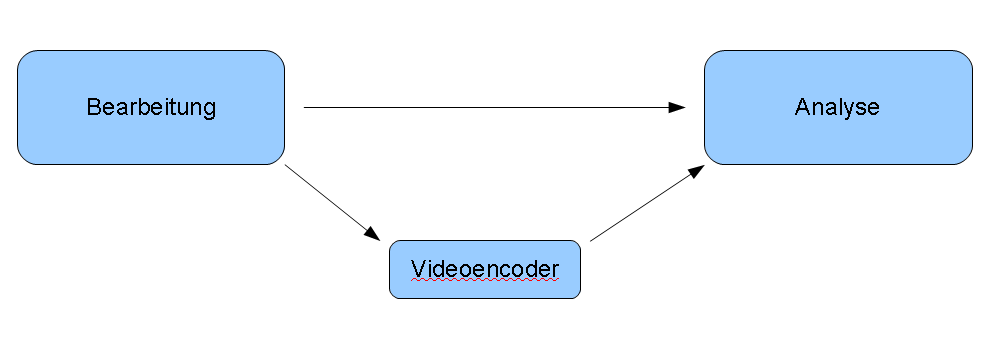
\includegraphics[scale=.35]{img/aufgabe.png}
		\vspace*{\fill} ~\\
	\end{center}
\end{frame}
\section{Architektur}
\begin{frame}
\frametitle{Architekturmuster  MVVM}
\begin{minipage}{5,5cm}
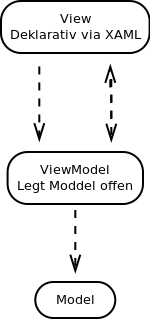
\includegraphics[scale=.5]{img/arch/mvvm.png}
\end{minipage}
\begin{minipage}{5,5cm}
\begin{itemize}
\item <+-> Model View ViewModel Architekturmuster.
\item <+-> View wurde nahezu vollständig deklarativ definiert.
\item <+-> Verbesserte Testbarkeit durch Trennung der Darstellung von der Anwendungslogik.
\end{itemize}
\end{minipage}
\end{frame}
\begin{frame}
\frametitle{Von der View zum ViewModel}
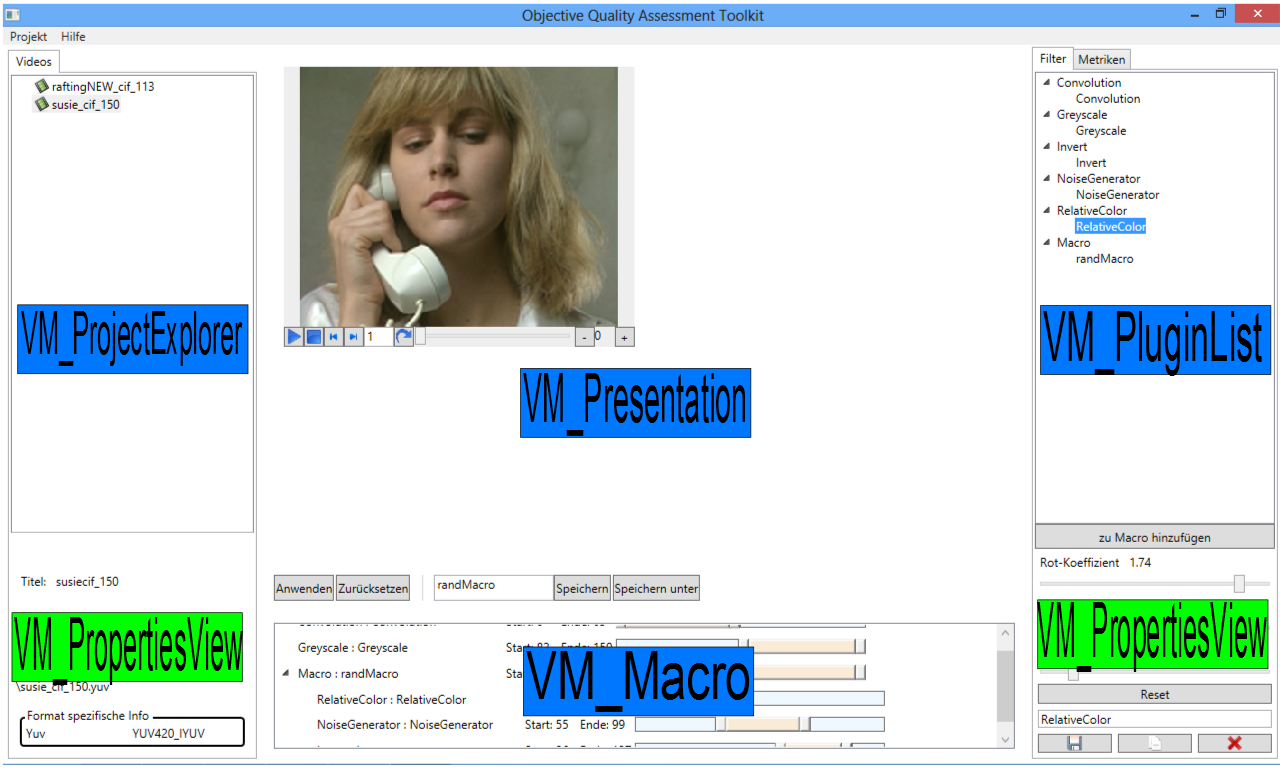
\includegraphics[scale=.23]{img/arch/generalOverview.png}
\end{frame}
\begin{frame}
\frametitle{Plugins}
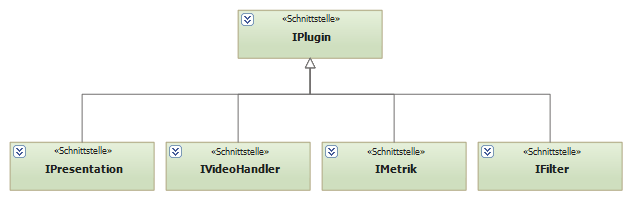
\includegraphics[scale=.5]{img/arch/IPluginStructure.png}
\newline
\newline
\begin{itemize}
\item <+-> Managed Extensibility Framework (MEF)
\item <+-> Plugins werden mit Hilfe exportierter Metadaten und
 implementierter Schnittstellen identifiziert
 \item <+-> Eine PluginManager Klasse ist für die Koordination und Konsistenz aller Plugins verantwortlich.
\end{itemize}
\end{frame}
\section{Entwicklungsumgebung}
\begin{frame}
	\frametitle{Entwicklungsumgebung}
	\begin{itemize}
	\item <+-> UML-Tool\\ Visual Studio 2010
	\item <+-> Entwicklungsumgebung\\ Visual Studio 2010
	\item <+-> Programmiersprache\\ C Sharp
	\item <+-> Code-Verwaltungssystem\\ Git
	\item <+-> Dokumenteneditor\\ TexMakerX
	\item <+-> Libraries\\
				AForge, Avalon, OxyPlot, 
				Managed Extensibility Framework
	\end{itemize}
\end{frame}
\section{Statistiken}
\begin{frame}
	\frametitle{Git Code Frequency}
	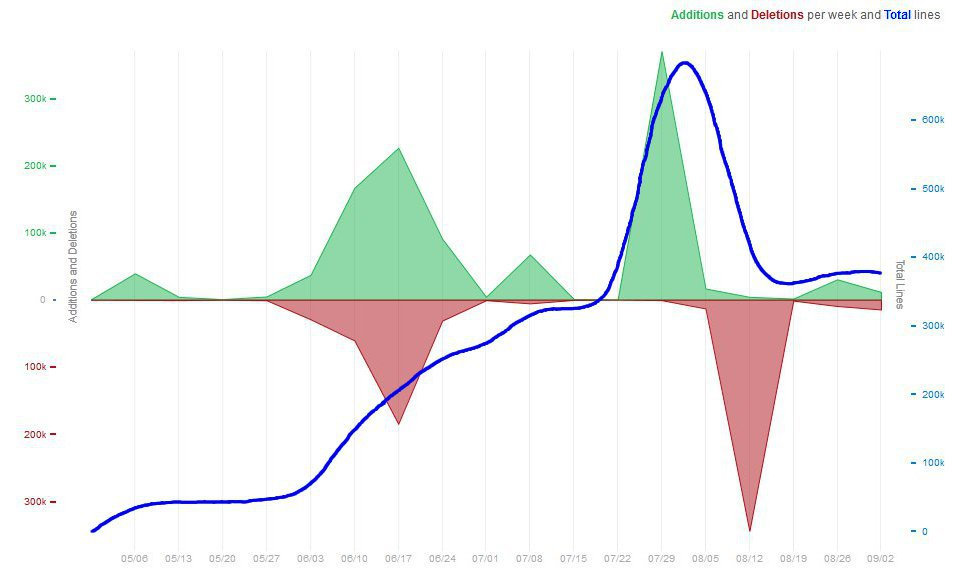
\includegraphics[scale=.33]{img/GitCodeFrequency.jpg}\\
	\hyperlink{Git Code Frequency}{https://github.com/PSE-2012/MMWTV/graphs/code-frequency}
\end{frame}
\begin{frame}
	\frametitle{Fun facts}
	\begin{itemize}
	\item <+-> 10667 Zeilen Code
	\item <+-> 82,5 Wartbarkeitsindex\\
	Nach Visual Studio gute Wartbarkeit
	\item <+-> Arbeitsspeicher zum analysieren von zwei Videos\\
	Für  QCIF(Abkürzung einer Auflösung) ca. 60MB
	\item <+-> 118 Issues 
	\item <+-> 843 Commits 
	\end{itemize}
\end{frame}
\section{Vorführung}
\section{Fazit}
%	-entwurf simpler machen sollen
%	-auf johannes höhren
%	-Binding toll aber frisst zeit
%	-c#
%	-einarbeitungzeit> rest
%	-teamwork(blöd gut optimal?)
\end{document} 
